%%%%%%%%%%%%%%%%%%%%%%%%%%%%%%%%%%%%%%%%%%%%%%%%%%%%%%%%%%%%%%%%%%%%%%%%%%%%%%%%%%%%%%%%%%%%%%%%%%%%%%%%%%%%%%%%%%%%%%%%%%%%%%%%%%%%%%%%%%%%%%%%%%%%%%%%%%%%%%%%%%%%%%%%%%%%%%%%%%%%%%%%%%%%
% Written By Michael Brodskiy
% Class: Fundamentals of Electronics
% Professor: M. Onabajo
%%%%%%%%%%%%%%%%%%%%%%%%%%%%%%%%%%%%%%%%%%%%%%%%%%%%%%%%%%%%%%%%%%%%%%%%%%%%%%%%%%%%%%%%%%%%%%%%%%%%%%%%%%%%%%%%%%%%%%%%%%%%%%%%%%%%%%%%%%%%%%%%%%%%%%%%%%%%%%%%%%%%%%%%%%%%%%%%%%%%%%%%%%%%

\documentclass[12pt]{article} 
\usepackage{alphalph}
\usepackage{tipa}
\usepackage[utf8]{inputenc}
\usepackage[russian,english]{babel}
\usepackage{titling}
\usepackage{amsmath}
\usepackage{graphicx}
\usepackage{enumitem}
\usepackage{amssymb}
\usepackage[super]{nth}
\usepackage{everysel}
\usepackage{ragged2e}
\usepackage{geometry}
\usepackage{multicol}
\usepackage{fancyhdr}
\usepackage{cancel}
\usepackage{siunitx}
\usepackage{physics}
\usepackage{tikz}
\usepackage{mathdots}
\usepackage{yhmath}
\usepackage{cancel}
\usepackage{color}
\usepackage{array}
\usepackage{multirow}
\usepackage{gensymb}
\usepackage{tabularx}
\usepackage{extarrows}
\usepackage{booktabs}
\usepackage{float}
\usepackage{mhchem}
\geometry{top=1.0in,bottom=1.0in,left=1.0in,right=1.0in}
\newcommand{\subtitle}[1]{%
  \posttitle{%
    \par\end{center}
    \begin{center}\large#1\end{center}
    \vskip0.5em}%

}
\usepackage{hyperref}
\hypersetup{
colorlinks=true,
linkcolor=blue,
filecolor=magenta,      
urlcolor=blue,
citecolor=blue,
}

\urlstyle{same}
\usepackage{fancyhdr}
\pagestyle{fancy}
\lhead[\textsc{Fall 2024}]{\textsc{Fall 2024}}
\chead[\textit{Electronics Exam 2 Equation Sheet}]{\textit{Electronics Exam 2 Equation Sheet}}
\rhead[\textsc{EECE2412}]{\textsc{EECE2412}}
\cfoot[\thepage]{\thepage}

\pagenumbering{gobble}
\begin{document}

\begin{multicols}{3}

  \begin{equation*}
    \text{Voltage Gain: }A_v=\frac{v_o}{v_i}
  \end{equation*}

  \begin{equation*}
    \text{Current Gain: }A_i=\frac{i_o}{i_i}
  \end{equation*}

  \begin{equation*}
    \text{Power Gain: }G=A_vA_i
  \end{equation*}

\end{multicols}

\vspace{-30pt}

\begin{multicols}{3}

  \begin{equation*}
    \text{Decibel: }A_{v\text{dB}}=20\log(|A_v|)
  \end{equation*}

  \begin{equation*}
    A_{i\text{dB}}=20\log(|A_i|)
  \end{equation*}

  \begin{equation*}
    G_{\text{dB}}=10\log(|G|)
  \end{equation*}

\end{multicols}

\vspace{-25pt}

$$\boxed{\text{Energy Conservation: }P_i+P_s=P_o+P_d\longrightarrow \left\{\begin{array}{ll} P_i&=\text{Power from Source}\\P_s&=\text{Power from DC Supplies}\\P_o&=\text{Output Power at Load}\\P_d&=\text{Power Dissipated in the Op-Amp}\\ \end{array}}$$

    \begin{center}
      \underline{Frequency Dependence:}
    \end{center}

    \vspace{-25pt}

  \begin{multicols}{2}

    \begin{equation*}
      \text{Capacitor: }Z_c=\frac{1}{j\omega C}
    \end{equation*}

    \begin{equation*}
      \text{Inductor: }Z_L=j\omega L
    \end{equation*}

  \end{multicols}

  \begin{center}
    \underline{Summing Point Constraint: }
  \end{center}
  \begin{itemize}
    \item Only applies when the op-amp is in negative feedback
    \item Assuming ideal op-amp, $V_+-V_-=0$ (no current at terminals)
    \item For non-ideal op-amps: $V_o=A(s)(V_+-V_-)$
  \end{itemize}

  \vspace{-25pt}

  \begin{multicols}{2}

    \begin{equation*}
      f_{3\text{dB}}=\frac{\omega_{3\text{dB}}}{2\pi}
    \end{equation*}

    \begin{equation*}
      \text{GBW}=|A_v||f_{3\text{dB}}
    \end{equation*}

  \end{multicols}

  \begin{center}
    \underline{Diodes:}
  \end{center}
  \begin{itemize}

    \item In Forward Bias (FB): Permit current flow, have a positive voltage drop

    \item In Reverse Bias (RB): No current flow (open circuit)

      \begin{itemize}

        \item Constant Voltage Drop (CVD): Diodes have same forward-bias drop ($\approx.7[\si{\volt}]$)

      \end{itemize}

    \item Assume bias mode for each diode in diagram, calculate values to verify assumptions

    \item CVD + resistance model: $r_d=\frac{nV_T}{I_{DQ}}$ (approximated around quiescent point, $Q$)

  \end{itemize}

  \vspace{-25pt}

  \begin{multicols}{4}

    \begin{equation*}
      I_D=I_se^{\frac{V_D}{nV_T}}+1
    \end{equation*}

    \begin{equation*}
      \text{Room Temp: }V_T\approx 26[\si{\milli\volt}]
    \end{equation*}

    \begin{equation*}
      \quad\quad\quad1<n<2
    \end{equation*}

    \begin{equation*}
      10^{-6} <I_s 10^{-18}[\si{\ampere}]
    \end{equation*}

  \end{multicols}

  \vspace{-25pt}

  $$\boxed{\text{\underline{Temp Dependence: }constant $I\to V$ drop decreases $\approx2[\si{\milli\volt}]$ per $1[\si{\celsius}]$ temperature increase}}$$

  Zener Diodes: $V_D=-V_{zo}-I_zr_z$ in breakdown, with $I_z=-I_D>0$\\

  Transformers: step voltages according to turns ratio ($N_p:N_s$) or ($n:1$), with $V_s=V_p/n$

  \begin{multicols}{2}

    \begin{center}
      \underline{BJT Regions}
    \end{center}

    \begin{center}
      \begin{tabular}[H]{|c|c|c|}
        \hline
        EBJ & CBJ & Mode\\
        \hline
        FB & RB & Active\\
        \hline
        FB & FB & Saturation\\
        \hline
        RB & RB & Cutoff\\
        \hline
      \end{tabular}
    \end{center}

    Note: When designing an amplifier confirm that the BJT is in the active region

    \begin{center}
      \underline{BJT Formulas}
    \end{center}
    \vspace{-10pt}
    $$I_E=I_C+I_B$$
    \vspace{-10pt}
    $$I_{E}=I_{ES}\left[ e^{\frac{V_{BE}}{V_T}}-1 \right]$$
    \vspace{-20pt}
    \begin{center}
      \underline{Active Region Only:}
    \end{center}
    \vspace{-10pt}
    $$I_C=\alpha I_E$$
    \vspace{-25pt}
    $$I_B=(1-\alpha)I_E$$
    \vspace{-25pt}
    $$I_C=\beta I_B$$
    \vspace{-25pt}
    $$I_S=\alpha I_{ES}$$

  \end{multicols}

  \vspace{-30pt}

  $$\boxed{\text{\underline{For BJTs:}} \quad\quad\beta=\frac{\alpha}{1-\alpha}\quad\quad\alpha=\frac{\beta}{1+\beta}\quad\quad\text{ Typically: }\alpha\approx 1\text{, and }I_C\approx I_E\text{ but }I_C<I_E}$$

  \begin{center}
    \underline{BJT Models}
  \end{center}

  \begin{multicols}{3}

    \begin{figure}[H]
      \centering
      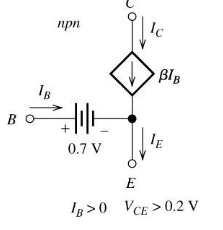
\includegraphics[width=.3\textwidth]{Figures/BJTActive}
      \vspace{-10pt}
      \caption{$npn$ in Active Mode}
      \label{fig:1}
    \end{figure}

    \begin{figure}[H]
      \centering
      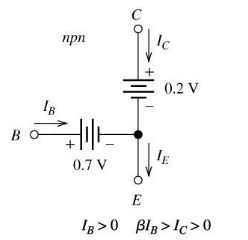
\includegraphics[width=.3\textwidth]{Figures/BJTSat}
      \caption{$npn$ in Saturation}
      \label{fig:2}
    \end{figure}

    \begin{figure}[H]
      \centering
      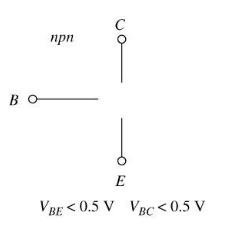
\includegraphics[width=.3\textwidth]{Figures/BJTCut}
      \caption{$npn$ in Cutoff}
      \label{fig:3}
    \end{figure}

  \end{multicols}

  \begin{multicols}{3}

    \begin{figure}[H]
      \centering
      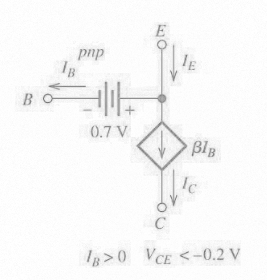
\includegraphics[width=.3\textwidth]{Figures/pnpActive}
      \vspace{-10pt}
      \caption{$pnp$ in Active Mode}
      \label{fig:4}
    \end{figure}

    \begin{figure}[H]
      \centering
      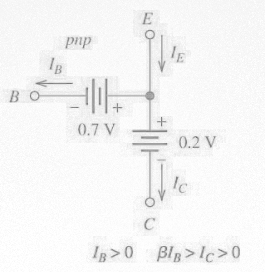
\includegraphics[width=.3\textwidth]{Figures/pnpSat}
      \caption{$pnp$ in Saturation}
      \label{fig:5}
    \end{figure}

    \begin{figure}[H]
      \centering
      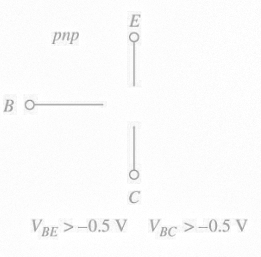
\includegraphics[width=.3\textwidth]{Figures/pnpCut}
      \caption{$pnp$ in Cutoff}
      \label{fig:6}
    \end{figure}

  \end{multicols}

  \newpage

  \begin{multicols}{2}

    \begin{figure}[H]
      \centering
      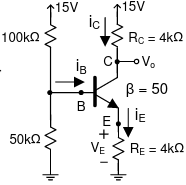
\includegraphics[width=.44\textwidth]{Figures/Four-Resista}
      \caption{Initial Circuit}
      \label{fig:7}
    \end{figure}

    \begin{figure}[H]
      \centering
      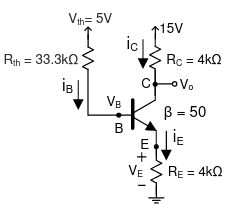
\includegraphics[width=.44\textwidth]{Figures/Four-Resistb}
      \caption{Th\'evenin Equivalent}
      \label{fig:8}
    \end{figure}

  \end{multicols}

\end{document}

